
 

Before running a user study, we test our hypothesis that topic
model overviews and active learning selection improve final cluster quality compared to standard baselines: list overview and random
selection. We simulate the four conditions on Congressional
Bills and 20 Newsgroups.

Since we believe annotators create more specific labels compared to the gold
labels, we use sub-labels as simulated user labels and labels as gold labels (we
give examples of labels and sub-labels in Section~\ref{sub:data}). We start with
two randomly selected documents that have different sub-labels, assign the
corresponding sub-labels, then add more labels based on each condition's
preference function (Section~\ref{sub:AL}).  We follow the condition's
preference function and incrementally add labels until 100 documents have been
labeled (100 documents are representative of what a human can label in about an
hour).  Given these labels, we compute purity, \abr{ri}, and \abr{nmi} over
time. This procedure is repeated fifteen times (to account for the randomness of
initial document selections and the preference functions with
randomness).\footnote{Synthetic experiment data available at
\let\hyper@linkurl\saved@hyper@linkurl
  \url{http://github.com/Pinafore/publications/tree/master/2016_acl_doclabel/data/synthetic_exp}
  \NoHyper
  }

Synthetic results validate our hypothesis that topic overview and active learning selection can help label a corpus more efficiently
(Figure~\ref{fig:syn_results}).  \abr{la} shows early gains, but
tends to falter eventually compared to both topic overview and topic overview  combined with active learning selection (\abr{tr} and \abr{ta}).

\begin{figure}[t!]
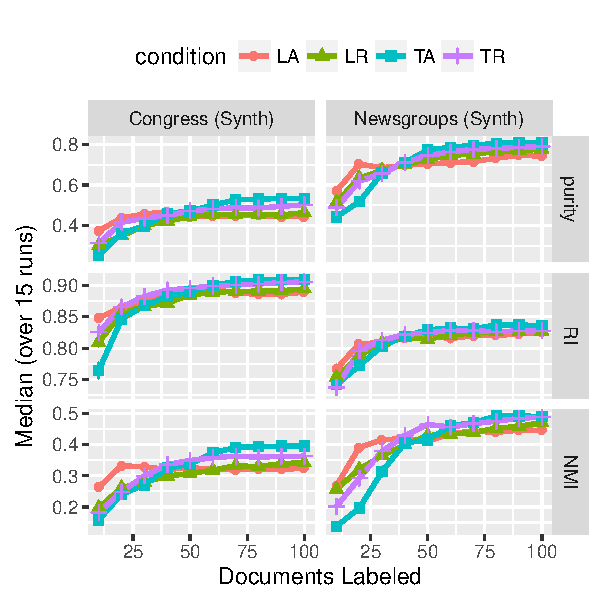
\includegraphics[width=\linewidth]{2016_acl_doclabel/auto_fig/synthetic}
\caption{Synthetic results on \abr{us} Congressional
  Bills and 20 Newsgroups data sets.  Topic models help guide annotation
  attention to diverse segments of the data.}
\label{fig:syn_results}
\end{figure}

However, these experiments do not validate \name{}.  Not all documents
require the same time or effort to label, and active learning focuses
on the hardest examples, which may confuse users.  Thus, we need to
evaluate how effectively actual users annotate a collection's
documents.
